% !TeX encoding = UTF-8
% !TeX root = MAIN.tex

%%%%%%%%%%%%%%%%
\chapter{Introduction}

Artificial Intelligence (AI) has undergone rapid development in the last few years. In today's modern era of mobile phones and computers, algorithms are used on a daily basis to have quick access to information and improve the efficiency of daily life.

While various algorithms (e.g.: Decision Trees, Linear Regression, Support Vector Machines, etc.), which are comprehensible by design, have been developed, the spotlight has turned to Deep Neural Networks (DNNs). This shift is attributed to the increase in computational power and the exponential increase in accessible data. Despite their remarkable accuracy, Deep Neural Networks remain opaque black boxes, which we struggle to understand \cite{Samek_2019}. Nevertheless, the immense improvement in performance and their ability to handle massive datasets have led to widespread adoption in contemporary devices \cite{zhang2022ai}. It is predicted, that algorithms based on Neural Networks will be becoming increasingly popular in the next years.

However, one of the primary difficulties with Neural Networks is the lack of reliable interpretability techniques. Understanding of the models is needed for various reasons: Regulatory laws require understandability of the data. The deficiency of interpretability in machine learning models leads to a presence of biases, such as gender discrimination and racial disparities. In the absence of a thorough understanding of a model's working, it becomes exceedingly difficult to confirm the functionality. This leads to users not trusting and avoiding machine learning systems. Beyond those user-centric advantages, it also supports the model development process and allows experts to extract valuable insights \cite{Samek_2019}.
 
Numerous interpretability methods have been developed, yet a universally reliable method remains missing. Particularly in the domain of image analysis, encompassing critical applications like automated driving and facial recognition, no solution is present. The decision-making rationale of neural networks remains unclear, attributed to factors like background elements, peripheral objects or lighting conditions. Efforts to address this issue have given rise to several gradient methods, aiming to assign significance values to pixels and represent their importance on neural network decisions \cite{Samek_2019}.

Another alternative option to mitigate the black-box nature of algorithms involves employing model-agnostic methods. These methods offer a computational linkage between features and labels, irrespective of which model is used. Although highly effective for smaller datasets, they begin to struggle as the data size and complexity increase. Because of this, they do not offer a reliable method to quickly make Neural Networks interpretable \cite{molnar2022}.

In light of these prevalent problems, the object of this thesis is to recapitulate interpretability methods for neural networks in computer vision. Emphasis is placed on the evaluation of post-hoc interpretability techniques, forecasting potential future developments and focusing on the strengths and weaknesses of distinct techniques. Concluding the theoretical segment, a practical demonstration showcasing the application of RemOve And Retrain (ROAR)\cite{hooker2019benchmark} is shown. 

\section{Structure of the Thesis}

\begin{enumerate}
	
	% TODO: - The structure could be slightly improved by stating about which section we currently talk about (e.g. In section X, we present...)
	\item In chapter \ref{sec:MLandI} "Machine Learning and their Interpretability", an overview of contemporary machine learning algorithms, categorizing them into two main groups: algorithms with inherent interpretability and those without. The goal is to make clear how supervised methods can be applied to image recognition tasks.
	\item In chapter \ref{sec:IoNN} "Interpretability of Supervised Machine Learning Algorithms" we delve into interpretability, emphasizing global and local model-agnostic techniques. These methods offer insights into overall model behaviour, regardless of algorithm specifics. 
	\item In subsequent sections \ref{sec:saliency} "Neural Network specific Interpretability Methods", model-specific post-hoc methods for Neural Networks are introduced. Feature visualization and gradient-based methods are explained.
	\item In chapter \ref{sec:evaluation} "Evaluation of post-hoc Interpretability methods", we focus on evaluating post-hoc interpretability methods. Various approaches to assess the effectiveness and dependability of these methods in offering meaningful insights into intricate models are introduced and discussed. Additionally, the advantages and disadvantages of these approaches are carefully examined to provide a comprehensive understanding of their applicability.
	\item In chapter \ref{sec:summary} "Which evaluation method and attribution method to use?", a conclusion is presented and an advice on which evaluation method to use is given. 
	\item In the last chapter \ref{sec:project} "Reconstructing ROAR", the practical application of the ROAR methodology using the Food-101 dataset \cite{bossard14} and MNIST dataset \cite{deng2012mnist} is presented to exemplify the discussed concepts. This real-world instance illustrates the current state of art of evaluation techniques in image recognition.
\end{enumerate}

%%%%%%%%%%%%%%%%
\chapter{Machine Learning and its Interpretability}
\label{sec:MLandI}

In the rapidly evolving landscape of machine learning, interpretability has emerged as an important concept. Before going in-depth into various algorithms and methods, the fundamental question of: "What is interpretable Machine Learning (IML) and why do we need it?" is answered.
\\
A broad definition of IML given by \cite{allen2023interpretable}: "Interpretable machine learning is the use of machine learning techniques to generate human-understandable insights into data, the learned model, or the model output." This definition underscores the important role of understanding complex models and allowing humans to understand the computation.
\\
% TODO reframe citation
Interpretability is important for various reasons, ranging from model validation and debugging to fostering validation and trust. Following key objectives have been identified: \cite{murdoch2019definitions} \cite{Roscher2020explainable} \cite{molnar2022} \cite{guidotti2018survey} \cite{lipton2017mythos} \cite{du2019techniques} \cite{carvalho2019machine} \cite{doshivelez2017rigorous}
\\\\
\textbf{Model Validation}: Interpretable models are essential for validating (by a human) whether a learned model behaves as expected and consistently aligns with prior expectations and knowledge about the system.
\\\\
\textbf{Model Debugging}: When unexpected behaviour occurs, finding the reasons for fault is impossible without understanding the system. Interpreting and understanding machine learning systems is critical for diagnosing, debugging and fixing systems \cite{koh2020understanding}. 
\\\\
\textbf{Transparency, Accountability \& Trust}: IML transforms black-box machine learning systems into understandable systems. The utilization of high-stakes societal applications requires accountability and trust in machine learning systems \cite{rudin2019stop} \cite{Samek_2019} \cite{xu2019inbook}. 
\\\\
\textbf{Ethics}: Machine learning algorithms can be trained on biased data leading to unfair predictions that are discriminatory. To improve the fairness of machine learning algorithms intepretable methods need to be deployed \cite{guidotti2018survey}. 
\\\\
\textbf{Data Exploration and Discovery}: Insights into major patterns, trends, groups, or artefacts of the data are achieved by applying human-interpretable techniques. These data exploration insights influence the data pre-processing and model decisions \cite{murdoch2019definitions} \cite{berkhin2006} \cite{tukey1981}. 




Before going into detail about the different methods of interpretability an overview of current supervised machine learning is given. Unsupervised machine learning is arguably intrinsically understandable, as the goal is to find a structure in the data. \cite{allen2023interpretable} With those examples, the necessity of interpretability for neural networks should be made evident.

\section{Supervised Machine Learning}

In supervised machine learning, there are a range of foundational classification methods. They are briefly introduced and analyzed for their interpretability. This section analyzes the base functionality of each algorithm. Furthermore, an analysis of the interpretability from a human perspective is made.
\\
The interpretability of algorithms depends on two factors, \cite{molnar2022}. When determining the transparency of an algorithm, we evaluate the human interpretability of how the model learns from the underlying structure of the data. Is it possible for a human to understand the implications of the mathematical operations? The second factor is the interpretability of the learned parameters. Understanding the factors of a linear regression model is easy. Grasping the millions of weights in a neural network is impossible.

In this section, we present a selection of frequently employed supervised machine learning techniques. As will become clear in the following subsections, interpretability was predominantly achieved through the methods' inherent interpretability.

\subsection{Linear Models}

When predicting outcomes, one of the simplest methods is to use a linear regression model. This model predicts by adding up n features ($x_n$) multiplied by an respective individual weight ($\alpha_n$). The predictive output $\hat{y}_i$ is calculated:

$$ \hat{y}_i= \alpha_0 + \alpha_1 x_1 + \alpha_2 x_2 +... +\alpha_n x_{n} + \epsilon$$

The alphas $\alpha_i$ indicate the significance of each feature. The initial coefficient $\alpha_0$ is known as the intercept, signifying the baseline. The noise $\epsilon$ describes the inevitable errors from inherent non-linearity in real-world dynamics or measurement inaccuracies.
\\
To train the model, the MSE-Loss (Mean Squared Error) or the ABS-Loss (Absolute Loss) is applied between the true label $y_i$ and the predicted label $\hat{y}_i$. The goal is to minimize this loss function. 

$$ \text{MSE-Loss} = \frac{1}{n} \sum_{i=1}^{n} (y_i - \hat{y}_i)^2$$
$$ \text{ABS-Loss} = \frac{1}{n} \sum_{i=1}^{n} |y_i - \hat{y}_i|$$
\\
The interpretation of the model is simple. The factors are described through the coefficient matrix. Each feature is distinctive to the model and the weighting is visible in the factors $\alpha_{i}$ (assuming normalization).

$$ \alpha = \begin{bmatrix}
	\alpha_0 & \\
	\alpha_1 & \\
	... & \\
	\alpha_i &
\end{bmatrix}
$$

Although linear models possess comprehensibility, provide a straightforward method for prediction and are inherently understandable, their application is limited to linear relationships and small datasets. In the domain of image recognition, it is not applicable because the features are not linearly correlated.

\subsection{Distance-based Methods}
\label{KNN}
K-Nearest Neighbors serves as a classification method by considering the nearest neighbours. 


Assume you have a dataset $D={(x_1,y_1),(x_2,y_2),…,(x_n,y_n)}$ where $x_i$ represents the feature vectors, and $y_i$ represents the corresponding class labels. Each $x_i$ is a point in a multidimensional feature space, and $y_i$ belongs to one of the classes (e.g., $y_i \in 0,1$) for binary classification). 
Given a new data point $x_{new}$ that you want to classify, K-NN works as follows:\\

1. Calculate the distance between $x_{new}$ and all other data points in the training dataset.\\
2. Select the K data points (nearest neighbors) with the smallest distances to $x_{new}$.\\
3. Count the number of data points in each class among the selected KK neighbors.\\
4. Assign $x_{new}$ to the class that has the majority of neighbors.\\

Although KNN's parameters are not interpretable by default, the underlying concept is straightforward: A sample has the same class as samples with similar features. This makes KNN's inherently interpretable and makes it a common choice when interpretability is needed. However, KNN's encounter difficulties when dealing with many features and larger datasets, therefore using it for image recognition is not recommended.

\subsection{Support Vector Machines}

Support Vector Machines (SVMs) \cite{boser1992training} are used to find a hyperplane that best separates different classes $y_i$ of data points. The primary objective is to maximise the distance between the hyperplane, defined by the weight vector $\vec{w}$, and the closest data points $x_i$ from each class. This is done to ensure that the   datasets are separated as much as possible. Because there may be classification errors and noise in the   dataset, it is possible to set an initial regularization parameter $C$ to handle outliers.

The optimization problem SVM in mathematical notion:

$$\text{Minimize } \frac{1}{2} \|\vec{w}\|^2 + C \sum_{i=1}^{n} \xi_i$$

$$\text{Subject to } y_i (\vec{w} \cdot x_i + b) \geq 1 - \xi_i, \quad \xi_i \geq 0 \text{ for } i = 1, \ldots, n$$

$\sum_{i=1}^{n} \xi_i$ represents the sum of slack variables ($\xi_i$), which measure how much a data point violates the margin constraint. While maximising the margin, Support Vector Machines (SVM) seeks to reduce this sum, minimizing the violations.\\
$ b $ is the bias term, which shifts the hyperplane away from the origin.

SVMs can handle non-linear data through the kernel trick, in which a kernel is applied to the data, transforming it to a different space before computing the hyperplane. However, as the dimensionality increases, SVMs become non-interpretable, making it challenging to visualize and understand the weight matrix. Moreover, SVMs struggle with larger datasets and high-dimensional feature spaces, making them less effective for image classification.


\subsection{Decision Trees}
\label{decision_tree}


Decision trees are a commonly used machine learning algorithm that proves effective in both classification and regression tasks. The reason for their popularity can be attributed to their user-friendly structure, which has the capacity to handle both categorical and continuous data. A decision tree is made up of three main types of nodes: root, internal, and leaf nodes, which combine to form a representation often depicted as a tree (see Figure 1).

\begin{figure}[h!]
	\centering
	\includegraphics[width=150mm]{figs/decision_tree}
	\caption[Decision Tree Example]{Decision Tree Example (created by Viktor Loreth)} 
	\label{fig:Decision_tree}
\end{figure}

The classes are separated in each root node by a decision criterion: $F_i$ <= criterion. The Gini impurity is commonly used for calculating the splitting criterion, which aims to best separate the data in the leaf. New nodes and are defined until the dataset is perfectly separated. However, this makes decision trees prone to overfitting as the model becomes overly complex and captures noise or random fluctuations in the training data, rather than the underlying patterns or relationships. Consequently, the resulting tree fits the training data exceptionally, but does not generalize well to new or unseen data. 

The depth of the tree can be restricted to avoid overfitting. Then, the majority is utilised to assign a label to the leaf. The depth of the tree can be restricted to avoid overfitting. Nevertheless, as the dimensionality grows, determining the depth becomes more and more challenging.

Random forests, comprise many decision trees and are known to prevent overfitting. However, they tend to be more challenging to interpret because of the use of multiple algorithms. Techniques like as SHAP values \cite{lundberg2017unified} or partial dependence plots \cite{PDP} can be employed to make them more understandable.
\\
Gradient boosting like XGBoost \cite{Chen_2016}, LightGBM \cite{Ke2017} and CatBoost \cite{prokhorenkova2019catboost} share similarities with random forests and decision trees, but they assign differential learned weights to each decision. They suffer from the same interpretability issues as random forests. While decision tree-based methods can be applied for image classification, their accuracy tends to be worse than in neural networks.


\subsection{Neural Networks}

The rise of neural networks and their powerful predictive capabilities has made them a popular choice for classification tasks. However, as these networks become increasingly complex, the traditional approach of understanding them through weight examination becomes challenging. With the emergence of Convolutional Neural Networks (CNN) in 2012 \cite{krizhevsky2012nn}, neural networks have become the state-of-the-art for image prediction.

n a neural network, each neuron calculates a weighted sum of its inputs and applies an activation function to produce an output. This output serves as the input for the subsequent layer. While various neuron types exist, including convolutional and recurrent neurons, foundational neurons are present in nearly all neural network architectures. A visual representation of a neural network can be seen in Figure \ref{fig:Neural_Network}.

\begin{figure}[h!]
	\centering
	\includegraphics[width=150mm]{figs/NeuralNetwork}
	\caption[Neural Network]{Neural Network (created by Viktor Loreth)} 
	\label{fig:Neural_Network}
\end{figure}

In this neural network, each circle, except those in the input layer, represents a weight matrix denoted as $w_{ji}$. Here, 'j' signifies the hidden layer number, and 'i' represents the weight number within that layer. The output of a neuron is determined by summing the products of the inputs $x_i$, their corresponding weights, and a bias term $b_{ji}$, expressed as $y_i = \sum_{i=1}^{n} w_{ji} \ast x_i + b_{ji}$. If the neuron is not in the output layer, an activation function, such as Sigmoid or ReLU, is applied to $y_i$, transforming it into $y_i = f(y_i)$. This transformed output of the neuron then becomes a new input $x_i$ for the next layer.

Labeled data is used to train a neural network. The prediction error is minimised by calculating the prediction error and the gradients. This is typically done by backpropagation over several epochs until the network can accurately predict new data.

Modern neural networks, such as ResNet50 \cite{he2015deep} comprise over 50 layers and utilize more than thousand kernels. Although they produce the greatest results, they lack an intuitive explanation of the learned parameters, unlike other types of supervised machine learning algorithms. Nonetheless, interpreting them to some degree is a necessity. Therefore, methods were developed which attempt to make any supervised machine learning algorithm interpretable. 

\chapter{Interpretability of Supervised Machine Learning Algorithms in Image Recognition}
\label{sec:IoNN}

Before going into detail of the chapter, the primary challenge of image recognition is explained:

Consider an image with dimensions of 3x224x224. The key objective in achieving model interpretability is to discern which elements of the image are responsible for influencing the model's output. This task is effectively illustrated as a simple version in figure \ref{fig:Task}. Some seemingly correlated data fields are creating a classification.

\begin{figure}[h!]
	\centering
	\includegraphics[width=150mm]{figs/TasktobeSolved}
	\caption[Image Classification]{Image Classification (created by Viktor Loreth)}
	\label{fig:Task}
\end{figure}

The task is to highlight or establishing a clear link between specific regions within the image and the output. The process of creating a correlation between image features and classification becomes exceedingly complex and non-linear for neural networks. This complexity explains why many interpretability methods often prove inadequate for image recognition. For instance, when an object within the image transitions from one quadrant to another, different pixels become responsible for the classification. Furthermore, challenges such as image blurriness or the presence of multiple potential classifications make interpretability even more difficult.

Before going into details of interpretability methods for this problem, a framework \ref{fig:IML_Overview} is presented \cite{allen2023interpretable} for classifying supervised machine learning methods and interpretability methods.

\begin{figure}[h!]
	\centering
	\includegraphics[width=100mm]{figs/Overview}
	\caption[Interpretability categorization \cite{allen2023interpretable}]{Interpretability categorization}
	\label{fig:IML_Overview}
\end{figure}

\textbf{Intrinsic vs Post-hoc}: Interpretability methods can be broadly classified into intrinsic and post-hoc techniques. Intrinsic methods are inherently understandable by design, while post-hoc interpretations involve analyzing the model's behaviour after its creation. Typical intrinsic understandable methods are Decision Trees \ref{decision_tree} and KNNs \ref{KNN}. 
\\
\textbf{Global Interpretations vs Local Interpretations}: Global Interpretations encompass the entirety of a fitted model. In contrast, local interpretations zoom in on specific portions of the model landscape, such as class boundaries.
\\
\textbf{Model-Specific Interpretations vs Model-Agnostic Interpretations}: 
Model-specific interpretations are tailored to a particular class of algorithms, like gradient methods for neural networks. In contrast, model-agnostic interpretations, such as LIME or SHAP, can be applied across any classification algorithm.

The goal of this section is to present several commonly used interpretability methods and evaluate their suitability for image classifications. As Neural Networks are the best performing methods for image recognition, the focus lies on the suitability of the interpretability methods for Neural networks. After going over different model-agnostic interpretability methods in the next section, we go in-depth about model-specific interpretations for neural networks in \ref{sec:nni}. 


\section{Global versus Local Model-Agnostic Methods}

When it comes to interpretability in image recognition, two broad categories of methods are commonly used: global model-agnostic methods and local model-agnostic methods. These methods are used to uncover the inner workings of complex models and provide a deeper understanding of the relationships between inputs and outputs. However, both global and local interpretability techniques face challenges, particularly in image recognition, which involves diverse and data-rich inputs, making interpretation a computationally demanding task. In the following subsection commonly used global and local model-agnostic methods are shortly explained and their suitability for image recognition is discussed.

\subsection{Global Model-Agnostic Methods}

The aim of global methods is to provide a complete overview of the functioning of a model. However, it is very difficult to represent the non-linearity in image classification for multiple classes. While some methods work reasonably well for the computation required, there is no global agnostic method that fully covers the need for interpretability.

\begin{enumerate}
	\item \textbf{Partial Dependency Plots:} Partial Dependency Plots (PDPs) are a straightforward method to display the relationship between individual or multiple features and an outcome. However, when dealing with a bigger feature size, there are too many plots to make sense out of the data. Therefore they are not feasible for Neural Networks and image recognition tasks \cite{PDP}.
	\item \textbf{Accumulated Local Effects:} Accumulated Local Effects (ALE) are an advancement of PDP. While it overcomes certain difficulties from PDPs, they struggle with the same problem when it comes to a bigger feature size.
	\item \textbf{Feature Interaction:} Feature Interaction analyzes the interaction between features inside the model. The underlying Friedman's H-statistic is a method to evaluate the correlation and variance. Because of the complexity of image tasks and the high computational costs, this method is not applicable to Neural Networks in a meaningful matter.
	\item \textbf{Functional Decomposition:} Functional Decomposition is commonly used in Neural Networks. In Chapter \ref{sec:network_dissection} a method to disassemble networks is presented.
	\item \textbf{Permutation Feature Importance:} Permutation Feature Importance is regularly used in visual machine learning tasks. In section \ref{pertubation} an example of a perturbation method is shown.
	\item \textbf{Prototype and Criticism:} The creation of clusters using the prototype and criticism method involves categorising well presented data instances as 'prototypes' and sparsely presented ones as 'criticism'. This approach aims to improves the interpretability of these clusters by verifying their classification accuracy. However, a significant challenge with this method arises when applying it to images, as it can be difficult to generate reliable clusters that effectively group the data.
\end{enumerate}


\subsection{Local Model-Agnostic Methods}

The aim of local methods is to reveal detailed knowledge of how a model behaves, often tailored to individual cases. In the field of image classification, where non-linearities and multiple classes contribute added complexity, achieving accurate interpretability for a single class is already challenging. Although some techniques effectively manage the trade-off between computational efficiency and interpretability in certain scenarios, there is currently no universally accepted model-agnostic method for achieving this.

\begin{enumerate}
	\item \textbf{LIME: Local Interpretable Model-agnostic Explanations:} Lime generates explanations in a local scope by training interpretable models on the predictions of a model. LIME only covers a single local context of the model. LIME can be applied to various types of data, including image data.
	\item \textbf{Scoped Rules (Anchors):} Anchors are distinctive patterns or conditions which guarantee a prediction. Finding anchors becomes increasingly expensive with more features present and is not normally used in neural networks. \cite{ribeiro2018}
	\item \textbf{Individual conditional expectation curves:} ICE's display one line per data sample and display how the sample changes when a feature changes. It is an individual version of PDP. \cite{goldstein2014peeking} It is not used in image classification or to evaluate neural networks.
	\item \textbf{Counterfactual explanations:} Counterfactual explanations of a prediction explain the smallest change of feature values which is necessary to change the prediction of an output. The problem in using this method is that for each instance multiple counterfactual explanations exist. (Rashomon effect) The use of counterfactual explanations in image recognition as a standalone method is not common.
	\item \textbf{SHAP (SHapley Additive exPlanations):} SHAP values \cite{lundberg2017unified} calculate how much each feature contributes to the difference between a models prediction for a specific instance and the average prediction across all instances. Positive SHAP values indicate features that increase the predicted likelihood for a particular class, while negative values indicate features that decrease it. It is used commonly in neural networks.
\end{enumerate}



\section{Model-Specific Interpretations for Neural Networks}
\label{sec:nni}
In the domain of Natural Language Processing (NLP) and Computer Vision, Deep Learning has proven very successful. By passing the features through a sequence of layers, characterized by matrix multiplications with kernel weights and nonlinear transformation functions, a prediction is computed. Depending on the specific task, additional elements like Long Short-Time Memory(LSTM) layers and Convolutional layers are utilized. Given the immense amount of mathematical operations and the non-linearity underlying a single prediction, humans are not fit to apprehend the mapping. To interpret predictions, we would have to decipher the intricate learned knowledge of numerous different kernels and weights.
Recognizing that humans cannot grasp millions of weights, the demand for interpretability methods is high. To assess the behaviour and predictions of Deep Neural networks, specific interpretability methods were developed. These methods calculate the likelihood of a feature being responsible for the result.
\\\\
While model-agnostic methods offer an approach to understanding Neural Networks, the sheer size of the data used to train and test Neural Networks makes this task extremely hard. For instance, in an image with the dimensions of 3x224x224, as commonly encountered in Food-101, the data features exceed 150.000. In NLP tasks, where vocabularies often encompass around 20.000 words, the computational complexity renders most model-agnostic techniques as too expensive.
\\
In the pursuit of comprehending the complexity of Deep Neural Networks, it makes sense to utilize the weights in the model. The information saved in the hidden layers as learned weights can be used to evaluate the network. Moreover, the gradients can be taken into consideration as well.
In the following subsections, several concepts for understanding Deep Neural Networks are introduced. 


\subsection{Feature Visualization}
\label{sec:network_dissection}

Feature Visualization tries to make parameters in singular layers in neural networks understandable. The goal is to give understanding of a deep neural network by dissecting each layer and understanding the underlying parameters through visualization.

The higher-level features in these networks relate to clear concepts, shown in Figure \ref{fig:feature-visualization}. As the features (image-pixels) pass through the layers, the feature changes at each layer. In each convolutional layer, the network gains new and more complex features. The smooth joining of fully connected layers then converts image-based data into predictions.
\\
\begin{figure}[H]
	\centering
	\includegraphics[width=150mm]{figs/FeatureVisualization}
	\caption[Network Dissection: Feature Visualization \cite{olah2017feature}]{Network Dissection: Feature Visualization }
	\label{fig:feature-visualization}
\end{figure}

The figure explains this process. The first convolutional layers find simple features like edges and basic textures. Later, they recognize more detailed patterns. The deepest layers learn about parts and objects. This object information passes to the other hidden layers, which then finally make a prediction.

Feature visualization is based on activating one kernel in the network. This involves maximizing the activation of a specific neuron (Visible in figure \ref*{fig:optimization}). There are two methods for achieving this. First, we can make use of the training image that triggers the highest activation. Yet, this approach faces a significant problem. When an image contains multiple objects, it is hard to pinpoint which object causes the activation. Because of this, an alternative route is adopted: generating new images from random noise. This is accomplished through methods like Generative Adversarial Networks (GANs) or other diffusion-based techniques.

\begin{figure}[H]
	\centering
	\includegraphics[width=150mm]{figs/ab}
	\caption[Activation Maximization\cite{olah2017feature}]{Activation Maximization}
	\label{fig:optimization}
\end{figure}

Feature visualisation provides a first insight into the behaviour of a model, improving the understanding of its inner layers. It also has the potential to enrich domain understanding by aligning learned features with domain-specific knowledge. Furthermore, it can assist in debugging and refining models, contributing to their overall performance improvement. However, interpretation of the visualised features is difficult and decision making is challenging to understand.

\subsection{Network Dissection}

Network dissection, a technique introduced by Olah in 2018\cite{olah2018the}, builds on the principles of feature visualization. This method establishes a link between individual kernels and the prediction of specific features by exploiting the concept of visualizing the importance of channels and kernels, as introduced in the section before.

Although this method is effective in comprehending low-level features, comprehending high-level features still remains a challenge. Furthermore, analyzing a single sample is very time consuming. However, this interpretability technique holds significant potential for enhancing the transparency of neural networks.


\subsection{Attribution Maps}
\label{sec:saliency}
Attribution maps are visualizations that highlight the regions of an input image that have the most significant impact on a models output. By revealing the areas that strongly influence a prediction, saliency maps bridge the gap between the models "black-box" nature and human understanding. An example attribution map is visible in figure \ref{fig:saliency}.

\begin{figure}[H]
	\centering
	\includegraphics[width=150mm]{figs/SaliencyExample}
	\caption[Attribution Map \cite{captum}]{Attribution Map}
	\label{fig:saliency}
\end{figure}

Attribution maps are typically calculated using SHAP\cite{lundberg2017unified} or gradient methods. Attribution maps provide a direct and intuitive way to understand which parts of input data influence a model's decision. The main difficulty is in generating reliable attribution maps. The remaining subsections introduce some commonly used methods. The key objective for all following methods is the same: Generating a reliable and easily understood attribution map.

\subsection{Visualising Image Classification Models and \& Deconv-Net}


Visualising image classification models (Gradient) \cite{simonyan2014deep} focuses on computing gradients within neural networks. It involves generating a forward pass of an image and then computing gradients for the class scores. These gradients are visualized, akin to the backpropagation process. However, this method faces two challenges. First, when Rectified Linear Units (ReLU) are used, negative gradients are seemed as unimportant and are set to zero. This leads to an information loss in the gradients. Second, in pooling layers, gradients are absent, resulting in further information loss.
\\
The Devonc-Net from Zeiler \cite{zeiler2013visualizing} addresses these problems:
A Deconv-Net-layer \cite{Zeiler2011AdaptiveDN} is attached to each convolutional layer providing a path back to the image pixels. The Devonc-Net practically learns weights to reverse the process from input to the last convolutional layer. Unpooling in Deconv-Net addresses the non-invertibility of pooling operations by preserving the original maxima locations through switch variables, which are subsequently employed to reconstruct the activations. To maintain positive signals during reconstruction, a reverse ReLU non-linearity is applied in each layer, similar to the forward pass. Additionally, Deconv-Net utilizes transposed filters, effectively mirroring each filter both vertically and horizontally to achieve filtering in the reverse direction.

This results in making it possible for visualizing the responsible input pixels for a classification output.

\subsection{Gradient-weighted Class Activation Map (Grad-CAM)}

Grad-CAM \cite{springenberg2015striving} ignores low-relevancy classes, which implies that percentages for predictions below a certain threshold are not taken into account. The method then backpropagates gradients specifically for the primary class of interest. These gradients are rescaled to fall within the [0,1] range and visualized. Grad-CAM takes into account all layers except for the convolutional layers. Evaluating the importance of each kernel before the convolutional layers offer insights into the significance of each input feature. This also explains the coarse accuracy, as pooling layers and convolutional layers are not handled and the resolution is up-scaled to the required format.

\subsection{Guided Grad-CAM}

Guided Grad-CAM combines the backpropagation \cite{springenberg2015striving} with another method to have a better localization. The up-sampled attribution map from Grad-Cam is multiplied with another attribution method. This acts as a lenses for other attribution methods to focus on specific parts of the attribution map.

\subsection{Integrated Gradient}
\label{IG}
Integrated Gradient \cite{sundararajan2017axiomatic} computes the integral of the gradients of the model's prediction with respect to its input variables. By integrating over this path, it quantifies how each feature contributes to the change in the model's prediction. A reference variable, such as a baseline is used to measure how each feature influences changes in each prediction. The method is commonly used, as it considers the entire input space and is applicable to any model.

\subsection{Ensemble Methods: Smooth Gradient, Smooth Grad² and VarGrad}

All the following methods can be applied to gradient-based techniques to adjust their behaviour and enhance their robustness in various applications.

\text{SmoothGrad} \cite{smilkov2017smoothgrad} is a smoothing approach to mitigates noise in gradient calculations. To achieve this, it generates a set of J noisy estimates by independently adding Gaussian noise $\theta$ to the input $x$. These noisy estimates are then averaged to obtain a more reliable and accurate gradient estimate, as represented by the formula. $g$ is describing the calculation of an attribution map, $A$, is the attribution map:

$$ A = \frac{1}{J}\sum_{i=1}^{J} (g(x+\theta))$$

\text{SmoothGrad²} \cite{hooker2019benchmark} builds upon the concept of SmoothGrad by squaring all estimates before averaging them. This modification is aimed at emphasizing the contributions of gradients while further reducing the impact of noise. The formula is as follows:

$$ A = \frac{1}{J}\sum_{i=1}^{J} (g(x+\theta)^2)$$

\text{VarGrad} \cite{adebayo2020sanity} offers an alternative approach to aggregating gradient estimates. Instead of summing them up or averaging them, VarGrad focuses on estimating the variance of these estimates. This aggregation provides insights into the variability of gradient information across different perturbations, offering a unique perspective on the model's behaviour. The formula for VarGrad is expressed as:

$$ A = Var(g(x+\theta))$$


%\subsection{Excitation Backpropagation}
%
%Excitation backpropagation\cite{zhang2018} focuses on a set of neurons within a neural network during the computational process. By doing so, it enables the combination of gradient information with the attribution maps, leading to precise object localization.
%
%The key feature of excitation backpropagation is the use of a probabilistic Winner-Takes-All (WTA) formulation. This formulation produces normalized attention maps, allowing for direct subtraction of these attention maps. This subtraction operation is crucial for highlighting the regions of interest within the neural network's activation, making it easier to understand which parts of the input data contribute most to a particular decision or classification.
%
%\begin{figure}[h!]
%	\centering
%	\includegraphics[width=150mm]{figs/TopDown}
%	\caption[CNN classifiers top-down attention map]{CNN classifiers top-down attention map \cite{zhang2018}}
%	\label{fig:topdown}
%\end{figure}
%
%The concept of identifying task-relevant neurons is central to Excitation Backprop. This involves evaluating the relative likelihood of a neuron "winning" against others within the same layer. Neurons with higher winning probabilities are deemed more relevant to the task at hand, and this information can be leveraged to understand the network's decision-making process and to localize objects or features within the input data.


%\begin{figure}[h!]
%	\centering
%	\includegraphics[width=150mm]{figs/DeterministicWTA}
%	\caption[Identifying task-relevant neurons in the network.]{Identifying task-relevant neurons in the network. The red shading of a dot indicates its relative likelihood of winning against the other ones in the same layer. \cite{zhang2018}}
%	\label{fig:taskrelevant}
%\end{figure}

\subsection{Summarizing Attribution Maps}

There exist many more attribution maps but there exists one major problem: There is no consensus which method should be used. While attribution maps have advantages \cite{molnar2022}, such that they are fast to compute and easy to interpret, they are also unreliable and can be insensitive to model and data. Furthermore, it is difficult to know whether an explanation is correct. In the next chapter, the evaluation of interpretability methods and metrics are discussed.


\newpage


\chapter{Evaluation of post-hoc Interpretability Methods \& Evaluation metrics}
\label{sec:evaluation}


In this chapter the evaluation of attribution maps and the underlying gradient methods is discussed. Finding suitable evaluation methods for attribution maps is difficult. Still, various evaluation methods have been developed which try to assess the performance of saliency methods. While they do not offer an objective truth if one saliency methods outperforms another one across all tests, they can offer some guidance one the effectiveness of saliency methods. Gupta\cite{gupta2022new} proposes that those evaluation methods can be broadly categorized into two types:

\textbf{Extrinsic Evaluation}: 
The evaluation is compared against predefined ground truths explanations, established by human annotator or by another network, as demonstrated in Zhang\cite{zhang2018}. However, the sheer amount of images makes the evaluation challenging. Furthermore, the quality of an attribution map is hard to judge. When is an evaluation correct? Also, Adebayo \cite{adebayo2020sanity} underscores the issue of confirmation bias, where an explanation may be considered correct, because it highlights the same regions as humans might choose, but not ensuring that the model employs the same learned concepts. Furthermore, in extrinsic evaluation a significant challenge is the lack of ground truths in attribution maps. Research still faces the challenge that the development of such a model is still missing.

\textbf{Intrinsic Evaluation}: 
Intrinsic methods rely on computational analyses within the neural network itself, without requiring human judgments. These methods are based on creating a new composite input using the heat map and the original input. Then they are evaluated using either the same model\cite{dabkowski2017real} or new model is trained and evaluated\cite{hooker2019benchmark}. While both these methods generate meaningful results, they both do not offer an objective evaluation method. Without re-training it is not clear if the degrade in performance stems from the distribution shift or the removal of informative features \cite{hooker2019benchmark}. By re-training, a different model is evaluated.
\\

Many interpretable AI-methods exist and there is a question: Can I compare the effectiviness between them? Can I combine the results and the one which seemingly has the most correlation is good? Neely, \cite{neely2021order} has tested several explainable AI methods in the domain of NLP and can only find little correlation. Additionally, the correlation is model and task dependent, which furthermore weakens this assumption. It is unclear however, if this result is the same in the task of image classification.
\\

After considering all these facts, it is not possible to meaningfully evaluate saliency methods by comparison or without violating fundamental assumptions. In the upcoming sections, potential evaluation metrics and methodologies are introduced to provide a more meaningful assessment. These metrics and methods do not fundamentally solve the problems, but they offer some guidance for evaluation.

\section{Completeness and Soundness}

In evaluation the composite input of the image $x \circ A$ describes an image with x\% (depending on the type of evaluation) of the pixels replaced by a grey value or the mean value. The pixels are chosen according to the highest or lowest values in the attribution map. Those inputs are then measured using intrinsic methods. The hypothesis is: If the not removed pixels are not important and the original net outputs the same labels, then the removed pixels are not important. This hypothesis is wrong, because the position of gray pixels can also be informative.
Gupta, 2022 \cite{gupta2022new} proposes Soundness and Completeness, which formalizes this problem and creates a numerical framework to evaluate the effectiveness of evaluating composition methods.

Soundness means: A certain portion of the image caused the net's output. x\% pixels are responsible for the classification of the label.\\
Completeness means: No matter which mask is chosen, as long as the x\% most important pixels are visible, the classification is correct.

This two metrics are useful to evaluate the correctness of masking. However, it is only a metric for other evaluation frameworks and is dependent on model and dataset. It is important to note however, because this metric was created in 2022 and is not included in any of the older papers. This information should give some background for the correctness of other older methods.

\section{Evaluating the Visualization of What a Deep Neural Network has learned}
\label{pertubation}

In the paper by Samek\cite{samek2017} a method is described, where the most important pixels detected by an attribution method are systematically replaced with randomly sampled values using a greedy algorithm. The objective is to measure the impact on the classification value f(x). The method can be applied with only removing the important pixels or by defining a local neighborhood around the pixel which is replaced as well. This neighborhood is defined, because from the context of the nearby pixels the same information can be deduced.

While the method produces results which confirm that removing important pixels leads to a performance drop, the models are not retrained. This leads to an evaluation of a different data distribution and therefore the results are not objective.

\section{A Benchmark for Interpretability Methods in Deep Neural Networks }

In this paper \cite{hooker2019benchmark} two methods to numerically evaluate saliency maps are presented. "RemOve And Retrain (ROAR)" and "Keep And Retrain (KAR)". This is done, by removing supposedly informative features from the input and observing the reaction of the neural network. In Section \ref{sec:project}, an example for MNIST and Food-101 is done.

% TODO: IMPROVE THE WHOLE Description
ROAR works as follows:
\begin{enumerate}
	\item \textbf{Selection of the most important pixels from an attribution map}\\
	An attribution map provides a mapping to the most important pixels. Those pixels are ranked based on their importance. For each attribution method, a map is calculated for each image. Depending on the method chosen, the absolute value can be taken to include pixels which highly advise against the classification.
	\item \textbf{ Replacement of x\% of the pixels with the mean value}\\
	In the ROAR algorithm, 10, 30, 50, 70 or 90 \% of the most important pixels are identified and replaced by the mean value. Both the training and the testing data undergo this process.
	\item \textbf{ Retraining the model using the modified dataset}\\
	To ensure that the data distribution of the dataset stays them same, retraining the model is necessary. Afterwards, the model is evaluated using several seed runs on the test set. The same split should be used for all runs. 
	\item \textbf{ Comparison of the attribution map with a random baseline} \\
	For each training setup, respectively with 0.1, 0.3, 0.5, 0.7 or 0.9 \% pixels replaced, a random baseline is considered, which generates random attribution maps for each image. This attribution maps are then used to replace the pixels and retrain the model as like the other methods. The random baseline is expected to perform worse than a sophisticated method.
	\item \textbf{ Evaluation} \\
	An attribution method is deemed effective if it consistently outperforms the random baseline across various setups.
\end{enumerate}

KAR operates similarly to ROAR, but instead of removing the most important pixels, the least important pixels are removed. Because KAR performs worse than ROAR, it is not described further.
\\
The conclusion of \cite{hooker2019benchmark} is that some commonly used attribution estimators like Gradient\cite{simonyan2014deep} , Integrated Gradient\cite{sundararajan2017axiomatic} and Guided Backpropagation\cite{springenberg2015striving} are worse than random assignments. On the other hand, the effectiveness of Smooth-Grad-Squared and VarGrad was confirmed. However, ROAR is sensitive to the   dataset used. While it does provide a numerical evaluation, it is sensitive to the model and   dataset used and therefore cannot independently and universally evaluate an algorithm.


\section{Benchmarking Attribution Methods (BAM)}
\label{sec:bam}
In practice, it is often challenging to determine the absolute importance of a feature. However, it is possible to calculate the relative importance of one feature concerning one model compared to another\cite{yang2019benchmarking}.\\

Given that one can calculate the relative importance, BAM\cite{yang2019benchmarking} comes to following assumption:
Consider an object which is described by $p_o$ pixels and a background described by the remaining pixels $p_s$. Each image has one object, and the remaining pixels are the background. If we train two classifiers, one to detect the objects and one to detect the scenes, then the relative feature importance of the $p_o$ pixels should be higher for the object classifier than for the scene classifier. Conversely, the $p_s$ pixels should be higher for the scene classifier than for the object classifier. To address the challenge of distribution shift, BAM carefully selects objects to insert that do not significantly alter the overall image distribution. For instance, objects with means similar to the dataset's mean are chosen. 

%todo Explain the BAM algorithm again;


%The BAM algorithm works as follows:
%\begin{enumerate}
%	\item \textbf{BAM dataset construction}\\
%	The BAM dataset is constructed by pasting object pixels from MSCOCO \cite{lin2015microsoft} into scene images from MiniPlaces \cite{zhou2016places}. An object is re-scaled to between 1/3 to 1/2 of a scene image at a randomly chosen location. The resulting images have an object label and a scene label. Either can be used to train a classifier. Every object class appears in every scene class and vice versa. Scenes which contain original BAM objects are not used.
%	\item \textbf{Common features and commonality}\\
%	Common features are defined as a set of pixels with semantic meaning (e.g. looks like a dog) which commonly appear in all examples of one or more classes. For example, a dog which appears in all bamboo forests is less common than a dog which appears in all images of bamboo forests, bedrooms and corn fields.
%	\item \textbf{Two Classifiers are trained and attribution maps are created}\\
%	An object detection classifier and a scene detection classifier are trained. Objects should be significantly more important than the scene to the object detector than to the scene detector. To verify this intuition, the objects are removed. With this knowledge, attribution maps can be tested by checking if the pixels are assigned noticeably higher attributions.
%	\item \textbf{Relative importance is calculated.}\\
%	With this knowledge, the object pixels should be more important than any other pixels for the detection classifier. Additionally, for the scene attribution, the attribution maps should be higher if the object pixels are replaced with the original pixels.
%\end{enumerate}


The advantage of BAM over ROAR \cite{hooker2019benchmark} and other methods is the lower computational cost. No retraining or perturbation is required. However, the method has the usual problems of evaluation algorithms: sensitivity to the dataset and model and not offering a universal truth.


\section{Sanity Checks for Saliency Maps}

Adebayo \cite{adebayo2020sanity} proposes two "sanity" tests to evaluate whether attribution methods are meaningful. It reveals that visual inspection by humans does not determine if the explanation is sensitive to the underlying model and data. Two instances of the framework are tested:
\\
The model \textbf{parameter randomization test} involves comparing the output of a saliency method on a trained model with the output of a randomly initialized untrained network of the same architecture. The output should differ, otherwise, the saliency map is considered ineffective. An example for this test is visible in figure \ref{fig:Sanity}. The \textbf{data randomization test} randomly shuffles the labels of the data. Afterwards, the model is trained on the altered   dataset. If the saliency maps do not differ from a normally trained model, then the method does not depend on the relationship of the images and labels.\\
\begin{figure}[H]
	\centering
	\includegraphics[width=150mm]{figs/Sanity}
	\caption[Cascading Randomization on Image Net\cite{adebayo2020sanity}]{Cascading Randomization on Image Net. The figure shows the original explanations. Progression from left to right indicates complete randomization of network weights up to that block inclusive. The last block corresponds to a network with completely reinitialized weights. }
	\label{fig:Sanity}
\end{figure}
If either of these two hypotheses fails during testing, the method under evaluation can be rejected, indicating that it fails a critical sanity check. On the tested methods, Guided BackProp \& Guided GradCAM fail the sanity checks.


\chapter{Which evaluation method and attribution method to use?}
\label{sec:summary}
Numerous attribution maps and possible evaluation methods have been looked at and it leaves data scientists with one question: Which evaluation method and attribution method should I choose?
\\
The unsatisfactory answer is: We do not know the answer yet. Depending on the model and   dataset used, different evaluation methods give varying outcomes. In Sanity check Adebayo \cite{adebayo2020sanity} and ROAR\cite{hooker2019benchmark} some methods were seen as unsuitable for the task considered. However, this was dependent on the model and the dataset. Considering there exists no ground truth for an evaluation method, there also is no ground truth for the attribution method. Opting for a SG - GRAD or a VAR-GRAD approach might result in favorable results for ROAR and Sanity checks. However, it remains difficult to evaluate visual explanations and there is no established ground truth to determine which evaluation method is the best. Consequently, further research is required to provide clearer guidance in this area.


%%%%%%%%%%%%%%%%

\chapter{Reconstructing ROAR} % 4 pages
\label{sec:project}

\section{Scientific Motivation and Goal}

% todo: rephrase

After looking at various methods in theory, we look at an approach ourselves in detail. A decided to look into ROAR\cite{hooker2019benchmark}, because it a relatively recently published study. We try to reproduce some experiments. Not all are looked into, because of the computational complexity. Additionally, we also want to look into the fluctuations between the different runs.


Due to resource constraints, the research was limited to evaluating food-101 \cite{bossard14} using two interpretability methods along a baseline model. Instead of five control runs, only four were made. As an initial proof-of-concept experiment the evaluation was done on the MNIST dataset\cite{deng2012mnist}.

\section{Project Setup MNIST}

Before starting a big computation on the food-101 dataset, the method was tested on a smaller dataset (MNIST) and only with one interpretability method. Integrated Gradient was chosen. The advantage of this setup is that the information loss is predictable by humans. By looking at the images with gray pixels, the information loss can be seen by human inspection. This information loss is visible as completely blank images and images with only very few white pixels. Those few pixels are the same for every image and therefore humans can make the assumption, that there exists no difference between the classes.


% Reframe the whole method to include the methodolgy in ROAR
A. Training the model

The model used in this report is a simple convolution neural network architecture consisting of two convolution layers, two pooling layers, and three linear layers. The model was trained for ten epochs with a learning rate of 1e-3 and an SGD optimizer with a momentum term of 0.9. The batch size was 64. Across five separate runs, the model achieved an average accuracy of 97.4\% with a standard deviation of 0.4\% on the test data. 

B. Dataset preparation and Splitting

% stopped here, redefine why MNIST was chosen
The MNIST dataset consists of 10 classes and 70.000 different images. It was chosen, because it is a small sized dataset and reconstructing the method is achieved easily. a) The importance of the pixels is clear from a human perspective. b) The model required to achieve a solid performance is very modest and speeds up the retraining. c) The information loss in retraining is visible in the pictures.\\

Furthermore, it is a small, simple dataset. The images are 28x28 pixels big and one pixel has a value ranging from [0,1] in gray-scale. The dataset used in this report was normalized using the mean and standard deviation and was split using the PyTorch library’s default splitting method (60.000 images for the training data, 10.000 images for the test data). This split has a fixed test and train set which include a homogeneous distribution of the classes. The training data was shuffled randomly using the inbuilt functions. The Cross entropy loss was selected for training runs. The same dataset split was used for all training runs to ensure consistency in the results.

C. Example of the modified dataset

The modified dataset is the result of combining the attribution map with the original image pixels $A \circ p$. In this operation the most x\% most important pixels are replaced with the mean value of the dataset.
In \ref{fig:IGvsRandom} the difference between Integrated Gradients and the Random Baseline is visible. In the first row, the random baseline is visible, in the second row the Integrated Gradient evaluation is shown. [10, 30, 50, 70, 90\%] of the pixels are blacked out (left to right).

\begin{figure}[h!]
	\centering
	\includegraphics[width=120mm]{figs/IGvsRandom}
	\caption{Integrated Gradients and Random Baseline Comparison}
	\label{fig:IGvsRandom}
\end{figure}

Judging by human intuition, Integrated Gradients appear to perform better overall thresholds. The model is expected to perform worse following retraining.

D. Retraining upon the new datasets

To ensure that the model learns consistently, the same split and learning parameters were utilized as in the standard case to retrain the model on the new dataset. An untrained network was created and then retrained for each training run. To validate the results and minimize the impact of random seed initialization, the training was performed with 5 different seeds and 5 models were created. In the Appendix, the exact results can be found.

E. Advantages and Disadvantages of the setup

Because of the small size of the dataset and the limited amount of classes, training a model is fast and effective. One disadvantage is the limited generalization of this setup for other datasets and models. The majority of use cases primarily involve working with images in the RGB colour space, utilizing deep learning models that are often more complex, and dealing with a larger number of distinct classes. Furthermore, the pixels themselves are blurred in their importance. In RGB images 3 channels are combined, which makes attribution maps more difficult to compute and understand.

F. Results

\begin{figure}[h!]
	\centering
	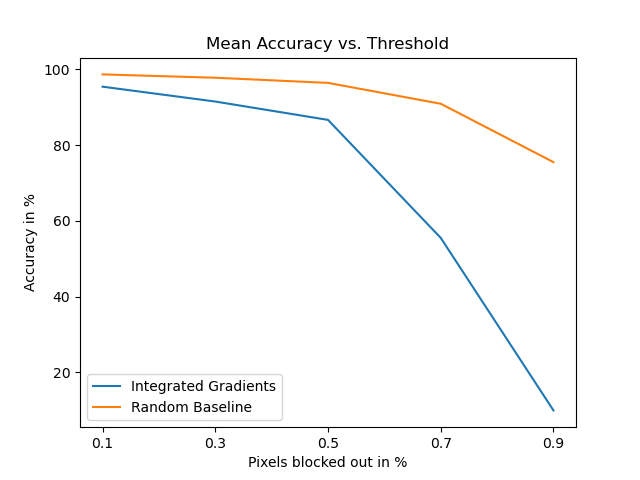
\includegraphics[width=150mm]{figs/mean_accuracy_vs_threshold}
	\caption{Accuracy: Random Baseline vs Integrated Gradient}
	\label{fig:Accuracy}
	
\end{figure}

Integrated Gradient is performing better than the random baseline.


\section{Project Setup Food-101}

The MNIST dataset \cite{deng2012mnist} was chosen as proof-of-concept. Because calculating the gradients and judging if a mask is meaningful is easier here, it should give a reliable baseline for the results. Only integrated gradients is tested, as is it only an example. 

A. Training the model

The model used in this report is ResNet50 \cite{he2015deep}. The Food-101 \cite{bossard14} dataset was chosen to replicate. The learning rate was adjusted to 0.175 and the batch size was chosen as 64. Using an SGD optimizer with momentum =0.9 and weight decay 0.0001 and a scheduler at epoch 30 with gamma=0.1, an accuracy of average 70.5\% with a standard deviation of 0.01 was achieved over 5 separate training runs on the test score. In total 31 epochs were done. 
By using this particular training setup, at the last epoch, the model learns more about the specific data. In the last epoch, an accuracy of 95\% on the training data was achieved.

In the original paper, an accuracy of 84.54\% was achieved on the Food-101 dataset. A smaller accuracy was achieved, as the training was noticeably shorter because only an NVIDIA GTX 1080 was available.

The data was resized with center-crop to make all images 3x224x224. Afterwards, they were normalized. No data augmentation like flips and mirroring was applied. The standard split 75:25 was applied. The saliency maps to generate the datasets were computed using the same models.

B. Results

\begin{figure}[h!]
	\centering
	\includegraphics[width=160mm]{figs/Acurracy Plots}
	\caption {Comparison of the accuracy behaviour of the original model vs the modified model.}
	\label{fig:Sanity}
\end{figure}

\begin{enumerate}
	\item In the random baseline the results of the original paper are confirmed. A drop in performance can be explained by the loss of information.
	\item In Integrated Gradient the results are also confirmed. But an unexpected behaviour occurs: The performance gets better by removing pixels. 
	\item The Guided Backprop result is also confirmed. But the behaviour is also unexpected. The performance is getting better by removing pixels.
\end{enumerate}



\section{Theoretical Implications}

Due to the fact, that the accuracy declines so slowly, it is unclear if the results given are really meaningful. Furthermore, there is no shared threshold when enough pixels are removed.
To provide a theoretical explanation for the implications of removing input dimensions on the resulting accuracy, the following factors should be considered:

\begin{enumerate}
	\item Input dimensions are removed and the accuracy drops:\\ The removed input was informative for the model and
	their absence reduces the ability of the model to identify the right class.
	
	\item We remove inputs and the accuracy does not drop.\\ (a) It is possible that the removed input dimensions	were not important for the model’s decision-making	process. The attribution map failed to identify important features, such as background pixels. (b) The input could be redundant and the information can be reconstructed using other available inputs. 
	
	\item We remove inputs and the accuracy increases:\\ The network removed consistent information which is available in the training set. By removing this pattern, over-fitting is reduced and the generalization improves.
\end{enumerate}


\section{Interpretation of the Results}

The main idea of ROAR was confirmed using the MNIST example. For simple datasets like MNIST, the concept can clearly be shown as meaningful.

The retraining performance of Food101 was partially confirmed, with a rise in accuracy by removing pixels contrary to the original runs.


The following questions are open:

- Is ROAR depending on the trained data and the dataset? Example: Using a dataset which does identify the species of animals. The face of the animal is clearly important. The eyes of the animals are also important. What is the relation of how important they are? How important is the zoom? Depending on the labels existing, the network learns different weights. In datasets like Birdsnap where the images are very common, only a small percentage of pixels are important and therefore blocking them out results in a lower accuracy.


- Does removing background pixels improve the accuracy because then the model focuses only on important patterns?
Well, this depends on the dataset.

- By removing information which is important through the correct label, maybe a pattern of recognition emerges.
All cakes have removed pixels at a position x. This could be the case for standardized pictures.

- Maybe removing the correct pixels to some degree makes it easier to recognize a pattern? For example, removing 50\% of the face and 50\% of the ears which are distinct to the species, more weight is given to the ears.



Knowing this -> Does ROAR still make sense?

While ROAR underlying logic makes sense, it is impossible to know whether the relation of a pixel makes sense and which patterns are learned. It does indeed offer an evaluation method, but the evaluation method in itself is not understandable. We do not know if the evaluation method does make sense, which simply moves the problem to a higher layer.




%%%%%

